\subsubsection{Ruční návrh}
\[
    I_D=\frac{1}{2} \cdot K P_N \cdot \frac{W}{L} \cdot\left(U_{G S}-U_{T H}\right)^2
\]
\[
    \frac{W}{L}=\frac{2\cdot I_{D}}{KP_{N}\cdot (U_{GS} -U_{TH})^2 } 
\]
\[
    \frac{W_{1} }{L_{1} }=\frac{2\cdot \num{25e-6}}{\num{220e-6}\cdot (\num{0.2})^2 } 
\]
\[
    \frac{W_{1} }{L_{1} }\doteq \num[round-mode=places,round-precision=2]{5.681818181818182} 
\]
Pro oba tranzistory zvolíme stejnou délku kanálu \(L_{1}=L_{2} = \qty{2}{\micro\meter}\), tedy \(W_{1} =\qty[round-mode=places,round-precision=2]{11,36363636363636}{\micro\meter}\). Druhý tranzistor má dosáhnout dvakrát vyššího proudu, takže zvolíme \(W_{2} =\qty{22,72}{\micro\meter}\).

\[
    R_1=\frac{U_R}{I_{M 1}}=\frac{U_{C C}-U_{G S 1}}{I_{M 1}}=\frac{U_{C C}-\left(U_{T H 0,1}+U_{O V, 1}\right)}{I_{M 1}}
\]
\[
    R_1=\frac{\num{1.8}-\left(\num{368,024e-3}+\num{0.2}\right)}{\num{25e-6}}
\]
\[
    R_{1} \doteq \qty{49,28}{\kilo\ohm}
\]

Výstupní odpor tohoto zapojení je roven výstupnímu odporu tranzistoru \(M2\): 
\[
    r_{O U T}=\frac{1}{\lambda \cdot I_{M 2}}
\]

\[
    r_{O U T}=\frac{1}{\num[round-mode=places,round-precision=3]{0,0437895} \cdot \num{50e-6}}
\]
\[
    r_{O U T}=\qty[round-mode=places,round-precision=3]{454,5454545454545}{\kilo\ohm}
\]

\subsubsection{Výstupní charakteristika}
\begin{figure}[h!]
    \centering
    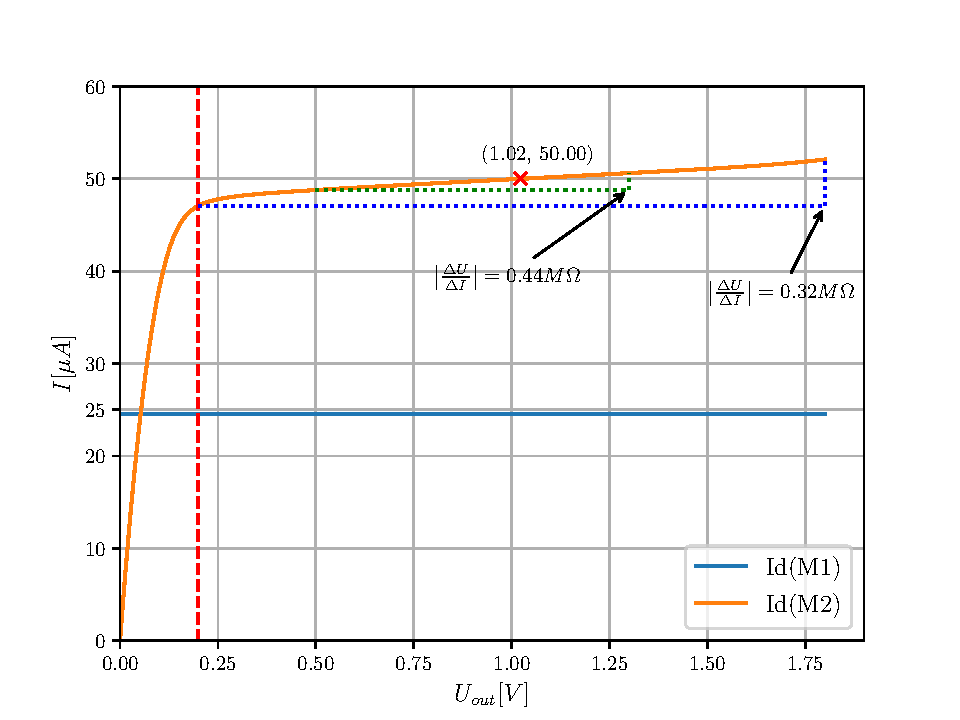
\includegraphics[width=0.8\textwidth]{2-1.pdf}
    \caption{DC analýza pro jednoduché proudové zrcadlo.}
    \label{fig:2-1-pdf}
\end{figure}

